\chapter{Расчет взаимодействия волноводов}
\label{coupling}

Для расчета эффективности взаимодействия двух волноводов необходимо знать распределения полей мод в каждом из них. Интегрально-оптические схемы, в основном, функционируют в одномодовом режиме поскольку в нем отсутствует межмодовая дисперсия и получается меньше помех, поэтому мы будем рассматривать только такие волноводы, в которых распространяется только основная мода. В ходе данной работы необходимо ставятся следующие задачи:
\begin{itemize}
	\item Смоделировать поля цилиндрического и планарного волновода в отдельности.
	\item Найти способ определения эффективности взаимодействия полей двух волноводов.
	\item Смоделировать изменения полей при поперечном, продольном и угловом смещении волноводов относительно друг друга.
\end{itemize} 
После решения поставленных задач можно будет сделать вывод о наиболее оптимальном взаимном положении волноводов и о том, насколько изменяется эффективность передачи при смещении их положения.

\section{Поле цилиндрического волновода}
\label{cylinder_field}
Как уже упоминалось ранее, цилиндрический волновод имеет следующее распределение поля (формула \ref{cylinder_bessel}):
$$
	H_z = H_0 J_v (\frac{ur}{a}).
$$
Для основной моды $v = 0$, а распределение можно считать гауссовым распределением. Сначала, учитывая  симметриею цилиндрического волновода рассмотрим проекцию поля на плоскость осевого сечения $xz$. В этом случае продольная составляющая будет зависеть только от $x$ и распределение можно описать формулой:
\begin{equation}
  \label{gauss}
  E(x)=\frac{1}{\omega\sqrt{2\pi}}\exp\left(-\frac{x^2}{2\omega^2}\right)
\end{equation}

Формула описывает нормальное распределение с вершиной в точке $x=0$.
Здесь $\omega = 1{,}1a$ - радиус моды, $a$ - радиус волновода. Соотношение соблюдается на длине волны, близкой к длине отсечки: $1 < \frac{\lambda}{\lambda_c} < 1.5$ \cite{lefevre}. Для моделирования возьмем несколько видов волокна:
\begin{itemize}
\item Corning SMF-28 ULL
\item Специальное волокно, разработанное для ВОГ на НИТИОМ
\item PANDA RCSM15-PS-U17B
\end{itemize}

\begin{figure}[h!]
	\begin{minipage}[h]{0.49\linewidth}
		\center{\includegraphics[width=1\linewidth]{img/distribution_courning.png} \\ а)}
	\end{minipage}
	\hfill
	\begin{minipage}[h]{0.49\linewidth}
		\center{\includegraphics[width=1\linewidth]{img/distribution_fog.png} \\ б)}
	\end{minipage}
	\vfill
	\begin{minipage}[h]{0.49\linewidth}
		\center{\includegraphics[width=1\linewidth]{img/distribution_panda.png} \\ в)}
	\end{minipage}
	\hfill
	\begin{minipage}[h]{0.49\linewidth}
	\end{minipage}
	\caption{Распределение поля в сечении волокна с разным радиусом моды: а)~Courning, б)~спец. волокно, в) PANDA}
	\label{diameter}
\end{figure}

Их технические характеристики представлены в таблице:
\begin{center}
\begin{tabular}{|p{6cm}|c|c|c|}
\hline
Модель & Corning & спец. волокно & PANDA \\
\hline
Вводимая длина волны, мкм & 1,55 & 1,55 & 1,55 \\
\hline
Диаметр оболочки, мкм & 125 & - & 165 \\
\hline
Радиус моды, мкм & 5,35 & 4,1 & 4,75 \\
\hline
Затухание на данной длине волны, дБ/км & 0,17 – 0,18 & - & 2.0 \\
\hline
\end{tabular}
\end{center}

Для сравнения, на рисунке \ref{diameter} показан вид распределения этих волноводов в сечении.

\section{Поле полоскового волновода}
\label{strip_field}
В качестве полоскового волновода для моделирования будем использовать титан-диффузионный оптический канальный волновод на подложке из монокристалла ниобата лития ($\rm Ti:LiNbO_3$)\cite{vlada}. Выберем  следующие параметры волновода: $W=12$ мкм; $H=8$ мкм; показатель преломления подложки $n_{be}=2,1383$; изменение показателя преломления в канале $\Delta n_{se}=0,01217$. Длину волны возьмем равной $\lambda = 1,55$ мкм. В итоге получилось следующее распределение.

\begin{figure}[h]
	\begin{minipage}[h]{0.49\linewidth}
		\center{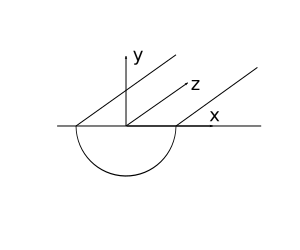
\includegraphics[width=1\linewidth]{img/polozok_isometry.pdf} \\ а)}
	\end{minipage}
	\hfill
	\begin{minipage}[h]{0.49\linewidth}
		\center{\includegraphics[width=1\linewidth]{img/strip_distribution.png} \\ б)}
	\end{minipage}
	\caption{а) общий вид канала, б) распределение поля в сечении}
	\label{polozok}
\end{figure}

\section{Эффективность передачи при поперечном смещении}

Целью данной работы является рассмотрение эффективности передачи энергии при соединении волноводов. Опишем эту зависимость теоретически.

Коэффициент передачи энергии определяется отношением скалярных квадратов мощности связанной волны к мощности входной волны \cite{lefevre}.

\begin{equation}
	\label{coupling_full}
	C = \frac{\left[\int\limits_{-\infty}^{\infty}E_{in}(x)e_{f0}^*(x) \,dx\right]^2}
	{\int\limits_{-\infty}^{\infty}e_{f0}(x)e_{f0}^*(x) \,dx
	 \int\limits_{-\infty}^{\infty}E_{in}(x)E_{in}^*(x) \,dx}
\end{equation}

\begin{figure}[h!]
	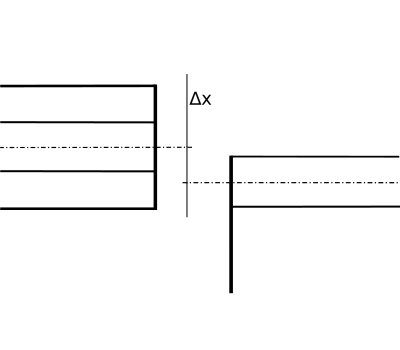
\includegraphics[width=.5\textwidth]{img/transverse_movement.pdf}
	\caption{Поперечное смещение волноводов}
	\label{transverse_movement}
\end{figure}

Рассмотрим изменение взаимного расположения полей в зависимости от поперечного смещения волноводов. В этом случае смещения по оси z не происходит, а значит значение комплексной части распределения не изменится и им можно пренебречь, а формула примет вид:

\begin{equation}
	\label{coupling_natural}
	C = \frac{\left[\int\limits_{-\infty}^{\infty}E_{in}(x)e_{f0}(x) \,dx\right]^2}
	{\int\limits_{-\infty}^{\infty}e_{f0}(x)^2 \,dx
	 \int\limits_{-\infty}^{\infty}E_{in}(x)^2 \,dx}
\end{equation}

Это выражение называется интегралом перекрытия  и показывает, какая часть энергии перейдет в возбуждение моды во втором волноводе. 

Рассмотрим поперечное смещение волноводов. При этом их поля также сместятся относительно друг друга и будут перекрываться не полностью.

\begin{figure}[h!]
	\includegraphics[width=.5\textwidth]{img/intersection.png}
	\caption{Распределение полей при поперечном смещении}
	\label{intersection}
\end{figure}

В показанном выше случае, поле возбуждаемой моды имеет максимум при $x=0$, а поле в входном волноводе имеет максимум в точке $x=4$. Из-за этого несоответствия в случае стыковки этих волноводов эффективность передачи будет небольшой, поскольку интеграл перекрытия этих полей равен 0.62. Очевидно что коэффициент передачи, то есть отношение интенсивности в выходном волноводе ко входному, максимален и равен 1 при условии $E_{in}~\equiv~e_{f0}$.

Рассмотрим стыковку канального волновода с оптическим волокном:

\begin{figure}[h!]
	\includegraphics[width=.5\textwidth]{img/intersection2.png}
	\caption{Перекрытие полей канального волновода и волокна}
\end{figure}

Распределение поля канального волновода сильно отличается от гауссиана, в отличие от распределения волокна, поэтому полной передачи энергии происходить не будет, ни при каком взаимном расположении волноводов.


\section{Продольное смещение волноводов}
Рассмотрим изменение эффективности передачи при продольном смещении волноводов. Возьмем полосковый волновод и оптическое волокно, которое будем перемещать относительно неподвижного полоскового волновода. Между волноводами образуется зазор, а, следовательно, имеет место расходимость гауссова пучка после выхода из волокна.
\begin{figure}[h!]
	\begin{minipage}[h]{0.49\linewidth}
		\center{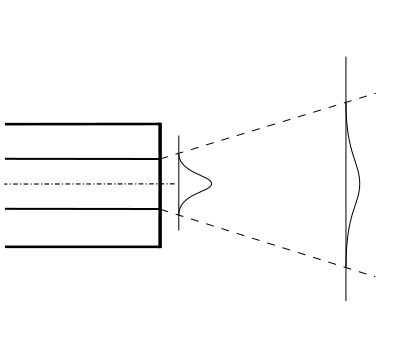
\includegraphics[width=1\linewidth]{img/gauss_divergence.pdf} \\ а)}
	\end{minipage}
	\hfill
	\begin{minipage}[h]{0.49\linewidth}
		\center{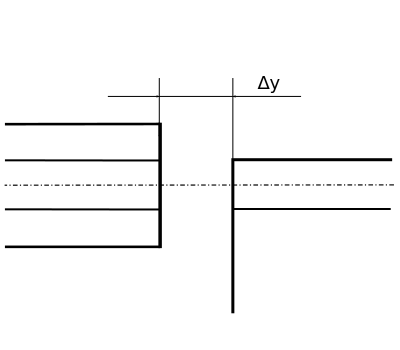
\includegraphics[width=1\linewidth]{img/longitudinal_movement.pdf} \\ б)}
	\end{minipage}
	\caption{а) расхождение пучка, б) схема продольного смещения}
\end{figure}

Пучок расходится под некоторым углом, который можно найти по формуле\cite{okamoto}:
\begin{equation}
	\Theta = \mathrm{arctg}(\frac{\lambda}{\pi n \omega_0})
\end{equation}
$\lambda$ - длина волны, $n$ - показатель преломления волновода, $\omega_0$ - радиус моды. При небольших углах расхождения можно упростить формулу:

\begin{equation}
	\Theta \approx \frac{\lambda}{\pi n \omega_0}
\end{equation}
Зная этот угол, можно найти радиус пучка на некотором расстоянии $z$:
\begin{equation}
	\omega(z) = \omega_0 + z\Theta = \omega_0 + \frac{\lambda}{\pi n \omega_0}z
\end{equation}

Вид распределения на некотором расстоянии можно найти, подставив в функцию (\ref{gauss}) получившееся значение $\omega$.

\section{Поле волноводов в пространстве}

Выше рассматривалась проекция распределения поля на плоскость. В пространстве гауссово распределение поля зависит от двух координат и равно:
\begin{equation}
  \label{gauss3d}
  E(x,y)=\frac{1}{2\pi\omega_1\omega_2}\exp\left(-\frac{x^2}{2\omega_1^2}-\frac{y^2}{2\omega_2^2}\right)
\end{equation}
где $\omega_1$ и $\omega_2$ - радиус моды по осям $x$ и $y$ соответственно. Вид такого распределения поля представлен на рисунке \ref{gauss3dPlot}.
\begin{figure}[h!]
	\includegraphics[width=0.5\textwidth]{img/gauss3d.png}
	\caption{Гауссово распределение в пространстве}
	\label{gauss3dPlot}
\end{figure}

Двухмерное распределение для планарного волновода будем строить из разложения функции по базису, описанного в работе\cite{vlada}.

Интеграл перекрытия также будет зависеть от двух переменных и примет вид:

\begin{equation}
	\label{coupling_2d}
	C = \frac{\left[\iint\limits_{-\infty}^{\infty}E_{in}(x,y)e_{f0}(x,y) \,dxdy\right]^2}
	{\iint\limits_{-\infty}^{\infty}e_{f0}(x,y)^2 \,dxdy
	 \iint\limits_{-\infty}^{\infty}E_{in}(x,y)^2 \,dxdy}
\end{equation}

\section{Угловое смещение волноводов}
Кроме описанных выше перемещений, возможен случай, когда волноводы стыкуются друг с другом не на одной линии, а под некоторым углом. При этом, для более плотного контакта, торец волокна скашивается под углом контакта. На рисунке \ref{angular_movement} показана схема такой стыковки.

\begin{figure}[h!]
	\begin{minipage}[h]{0.49\linewidth}
		\center{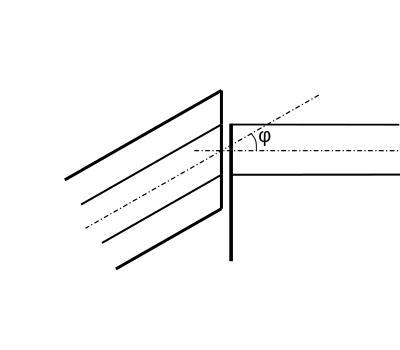
\includegraphics[width=1\linewidth]{img/angular_movement.pdf} \\ а)}
	\end{minipage}
	\hfill
	\begin{minipage}[h]{0.49\linewidth}
		\center{\includegraphics[width=1\linewidth]{img/wg_cutoff.png} \\ б)}
	\end{minipage}
	\caption{Угловое смещение волноводов а)~схема стыковки, б)~вид волокна со сколом}
	\label{angular_movement}
\end{figure}

В этом случае площадь контакта увеличивается, а вид распределения на выходе из волокна становится эллиптическим. В случае контакта параллельно плоскости скола изменяется только большая полуось, малая остается равной радиусу волокна. Изменение большой полуоси эллипса $r_1$ зависит от угла стыковки $\varphi$, а, следовательно, и угла скола. Ее можно найти по следующей формуле:
\begin{equation}
	r_1 = \frac{r}{\cos \varphi}
	\label{ellipse_axis}
\end{equation}
Учитывая, что радиус моды пропорционален радиусу волокна, можно написать аналогичное выражение для радиусов мод. Пусть $\omega_1$ - радиус моды по большой полуоси, $\omega_2$ - радиус моды по малой полуоси, равный исходному радиусу моды $\omega$
\begin{equation}
	\omega_1 = \frac{\omega}{\cos \varphi}
	\label{ellipse_axis}
\end{equation}
В итоге получим гауссово распределение такого волновода:
\begin{equation}
  E(x,y)=\frac{1}{2\pi\omega_1\omega_2}\exp\left(-\frac{x^2}{2\omega_1^2}-\frac{y^2}{2\omega_2^2}\right)
\end{equation}